\subsection{Buying a vehicle-sharing or a public transport service}
The user, for some tasks, maybe wants to take a bus or another public transport service. Furthermore, in Milan there are lots of alternatives to public transport, such as the car-sharing or the bike-sharing services, so the user might want to use one of these to reach a task location. For this reason, the \emph{Travlendar+} System, not only support the user in the process of choosing and buying a possible ticket from the public transport site or application, but also redirects the user to the right place where to book and rent a shared based travel mean service.

\begin{table}[H]
	\centering
    
    \begin{tabular}{|p{3.5cm}|p{10.3cm}|}
    
    \hline
    \textbf{\large{Actors}}  			& \tabitem User\\
                                        & \tabitem Car-Sharing Service\\
                                        & \tabitem Bike-Sharing Service\\
                                        & \tabitem Public Transport Service\\
                                        
    \hline
    \textbf{\large{Goals}} 				& \ref{goal:travel} \ref{goal:buyTicket}\\
    
    \hline
    \textbf{\large{Enter Condition}}	& The user should be logged in the                                                        \emph{Travlendar+} system and the calendar should be already scheduled\\
    
    \hline
    \textbf{\large{Events Flow}}		& \begin{enumerate}[leftmargin=0.5cm]
                                          	\item The user select a task
                                          	\item The user press the "Show Transport Information" button
                                          	\item The user select the type of transport service he wants to use
                                          	\item The user then selects if he wants to buy the ticket
                                          \end{enumerate}
    										\\
    \hline
    \textbf{\large{Exit Condition}} 	& The user should confirm the operation, then the system redirects he to the correct site of the selected service: Car-Sharing, Bike-Sharing or Public Transport\\
    
    \hline
    \textbf{\large{Exception}} 			& \\
    
    \hline
    
    
    \end{tabular}
	
\end{table}

\begin{figure}[H]
\centering
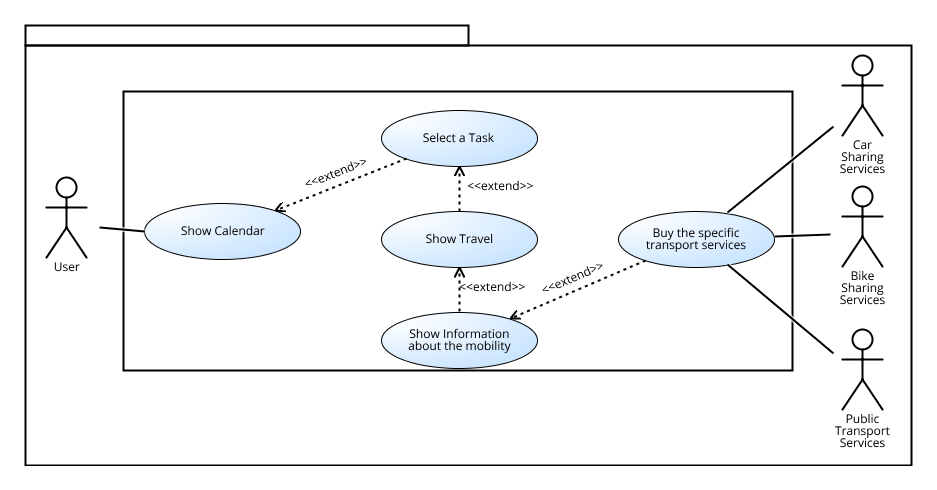
\includegraphics[scale=0.5]{Pictures/UseCaseDiagram/Buy_services.png}
\caption{UML Use Case Diagram for buying services operation DA RENDERE COERENTE CON SHOW TRANSPORT INFO: SHOW CAL, SHOW TASK, SHOW TRAV INFO... VEDI ANCHE UML DI MODIFY TASK: CHANGE TASK PREF E SHOW INFO}
\end{figure}
